\section{Digital Signal Processing}

In this section, it will be discussed how the digital audio signal was processed and recognized. 

The digital signal processing is divided into three main parts: I2S input, audio processing, and I2S output. The I2S input is responsible for receiving the digital audio signal from the microphone. The signal processing is responsible for processing the digital audio signal, and the I2S output is responsible for sending the processed digital audio signal to the speaker. In figure \ref{fig:DigitalInterface} is shown the block diagram of the digital signal processing.

\begin{figure}[H]
    \centering
    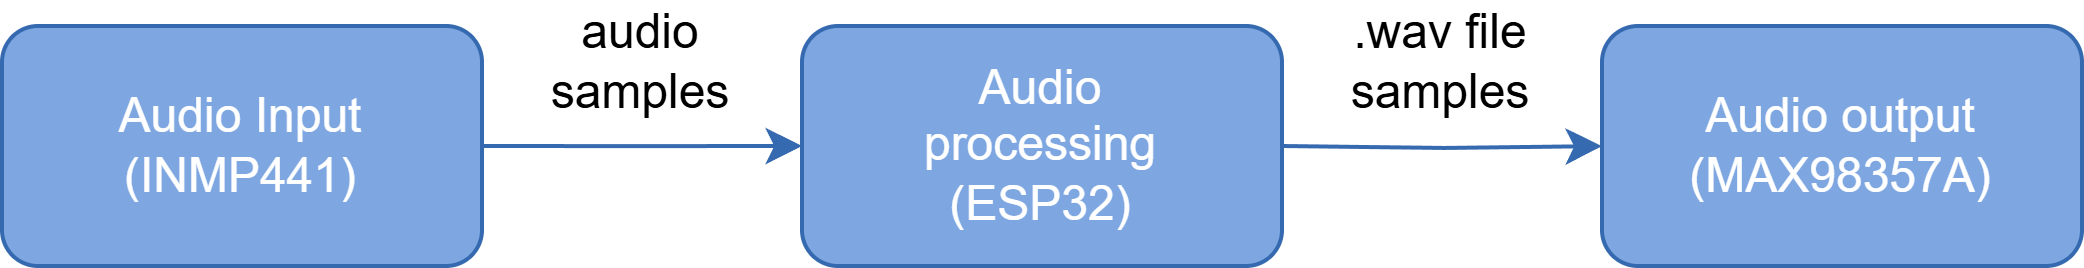
\includegraphics[width=0.8\textwidth]{Images/audio_processing_diagraampng.png}
    \caption{Block diagram of the digital signal processing.}
    \label{fig:DigitalInterface}
\end{figure}

\subsection{I2S DMA Buffer}

The DMA buffer (Direct Memory Access buffer) is a memory region used to transfer data between the I2S peripheral and the main memory without continuous CPU intervention. It is crucial for managing high-speed data streams, such as audio, ensuring efficient operation.

In reception (Audio Input), the DMA buffer acts as an intermediate storage area where data received by the microphone is temporarily stored before being processed by the application. 

The process of the DMA buffer in reception is:
\begin{enumerate}
    \item The I2S receives serialized audio data from the microphone.
    \item The DMA writes this data into the buffer.
    \item When the buffer is full, the audio processor (program) processes the data.
\end{enumerate}

To have a continuous audio retrieval, it was implemented a circular buffer. When the buffer is full, the DMA continues to write data to the buffer, overwriting the oldest data. This way, the audio processor can continuously process the audio data without interruptions.

In transmission, the DMA buffer is filled with data to be sent. The DMA reads the data from the buffer and automatically transfers it to the I2S amplifier, which transmits it to the speaker.

The process of the DMA buffer in transmission is:
\begin{enumerate}
    \item The WAV reader (program) writes data to the buffer.
    \item The DMA transfers data from the buffer to the I2S peripheral.
    \item The I2S transmits the serialized data to the speaker.
    \item When the buffer is empty, an event or interrupt is triggered to load new data for transmission.
\end{enumerate}

\subsection{Audio Input}

The audio input was done with a I2S MEMS (Micro-Electro-Mechanical System) breakout board (INMP441) that sends the audio signal in I2S format. The I2S format is a serial protocol that is used to transmit audio data and has three lines: the bit clock (BCLK), the word select (WS), and the data line (DIN). 
\begin{itemize}
    \item BCLK: The bit clock is the serial clock that is used to synchronize the data transmission from a peripheral.
    \item WS: The word select line indicates if the data is sent or received from left or right channels.
    \item DIN: The data line carries the audio data.
\end{itemize}

A diagram of the I2S format is shown in figure \ref{fig:I2S}.

\begin{figure}[H]
    \centering
    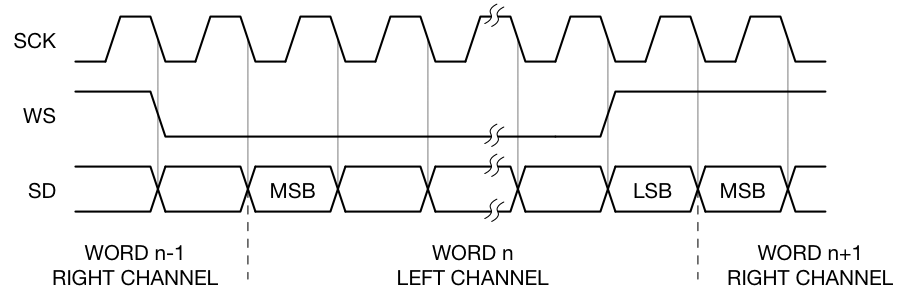
\includegraphics[width=0.8\textwidth]{Images/i2s.png}
    \caption{I2S format.}
    \label{fig:I2S}
\end{figure}

The I2S MEMS breakout board is a interesting for this application because it integrates an audio amplifier, ADC and the I2S interface. Thus, the output from the board can be fed directly into the ESP32 without using the internal ADC of the ESP32.

To configure the communication the I2S MEMS breakout board was set to record audio from right channel, 32 bits per sample and a sample rate of \SI{16}{\kilo \hertz} that is suitable for voice recording. 

\subsection{Audio Output}

The audio output was obtained with a MAX98357A I2S Class D amplifier that receives the audio signal in I2S format and outputs the audio signal to the speaker. The MAX98357A is a low-cost, low-power mono audio amplifier that is suitable for this application. The MAX98357A has a built-in DAC and PWM modulator that converts the digital audio signal to an analog audio signal. 

The MAX98357A was configured to receive the audio signal in both channels right and left, 16 bits per sample per channel and a sample rate of \SI{16}{\kilo \hertz} that is suitable for voice reproduction, the two channels were mixed to output the audio signal to the speaker because in this application it was only used one speaker.

The amount of power that the MAX98357A can deliver is limited by the speaker impedance. The MAX98357A can deliver up to \SI{1}{\watt} of power to a \SI{8}{\ohm} speaker with a power supply voltage of \SI{5}{\volt}. 

To maximize the gain of the MAX98357, a pull down resistor of \SI{100}{\kilo \ohm} was connected to the gain pin of the amplifier.

The class D amplifiers are also known as switching amplifiers because they operate by rapidly switching the output transistors on and off, they output a modulated signal that switches between the positive and negative power rails. The signal is passed to a speaker to recover the audio signal. This makes the amplifier very efficient as the transistors are only dissipating power when they are switching from high to low and low to high.

\subsection{Audio Processor}

The audio processing was done with the ESP32 microcontroller that receives the digital audio signal from the I2S MEMS breakout board, processes the audio signal and sends the processed to the prediction model.

The audio processor has to recreate the same process that was used for the training data and then convert the audio signal to a spectrogram.  

The process involved was:
\begin{itemize}
    \item Find the minimum and maximum values of the samples.
    \item Normalize the samples.
    \item Copy the samples to the FFT input buffer.
    \item Apply a hamming window to the samples.
    \item Perform the FFT.
    \item Extract the energy in which frequency bin.
    \item Average pooling process similar to the one used in the training data.
    \item Take the logarithms of the values that give reasonable values to feed into the model.
\end{itemize}

The spectrogram to a mel spectrogram that is a spectrogram where the frequencies are converted to the mel scale that is a perceptual scale of pitches that is based on how humans perceive sound. The audio processor has to convert the mel spectrogram to a MFCC (Mel-frequency cepstral coefficients) that are coefficients that collectively make up an MFC. The MFCC is a representation of the short-term power spectrum of a sound that is based on a linear cosine transform of a log power spectrum on a nonlinear mel scale of frequency.


\section{Digital Audio Recognition}

To detect and recognize commands from the audio signal, a mechanism with to types of recognition was designed: recognition with a machine learning model implemented in the ESP32 using TensorFlow Lite and recognition outsourcing the process to the Wit.ai platform.

\subsection{Model and TensorFlow Lite} 

The machine learning model was trained with the Google Speech Commands dataset that contains 65,000 one-second long utterances of 30 short words. The model was trained to detect the presence of a word in the audio signal. 

The model was trained with a convolutional neural network of an open sourced Jupyter notebook, that predicts the presence of a word in the audio signal by analyzing the spectrogram of it. Then the trained model was converted to C code to be implemented in the ESP32.

The TensorFlow Lite library was used to implement the voice activity detection algorithm of the machine learning model. The TensorFlow Lite library is a lightweight version of the TensorFlow library that is optimized for mobile and embedded devices. 

\subsection{Neural Network}

The neural network as the functions to communicate with the model obtained(load an input and make a prediction).

\subsection{Interact with Wit.ai}

The Wit.ai platform allows the development of voice recognition applications that can be used in the project. It has a REST API that allows the application to send audio data to the platform and receive the recognized text. The Wit.ai platform uses machine learning algorithms to recognize the speech and convert it to text. 

To interact with the Wit.ai platform, the application has to send a POST request to the platform with the audio data. The platform will process the audio data and return the recognized text. To avoid having to buffer the entire audio sample in memory a chuncked a upload of the data was performed.

A connection to wit.ai is created and then chuncks of data are uploaded until it collects sufficient audio to capture the user´s command. After that the results are returned from the API and the important relevant information is extracted (intent, name).


